\documentclass{article}\usepackage[]{graphicx}\usepackage[]{color}
%% maxwidth is the original width if it is less than linewidth
%% otherwise use linewidth (to make sure the graphics do not exceed the margin)
\makeatletter
\def\maxwidth{ %
  \ifdim\Gin@nat@width>\linewidth
    \linewidth
  \else
    \Gin@nat@width
  \fi
}
\makeatother

\definecolor{fgcolor}{rgb}{0.345, 0.345, 0.345}
\newcommand{\hlnum}[1]{\textcolor[rgb]{0.686,0.059,0.569}{#1}}%
\newcommand{\hlstr}[1]{\textcolor[rgb]{0.192,0.494,0.8}{#1}}%
\newcommand{\hlcom}[1]{\textcolor[rgb]{0.678,0.584,0.686}{\textit{#1}}}%
\newcommand{\hlopt}[1]{\textcolor[rgb]{0,0,0}{#1}}%
\newcommand{\hlstd}[1]{\textcolor[rgb]{0.345,0.345,0.345}{#1}}%
\newcommand{\hlkwa}[1]{\textcolor[rgb]{0.161,0.373,0.58}{\textbf{#1}}}%
\newcommand{\hlkwb}[1]{\textcolor[rgb]{0.69,0.353,0.396}{#1}}%
\newcommand{\hlkwc}[1]{\textcolor[rgb]{0.333,0.667,0.333}{#1}}%
\newcommand{\hlkwd}[1]{\textcolor[rgb]{0.737,0.353,0.396}{\textbf{#1}}}%
\let\hlipl\hlkwb

\usepackage{framed}
\makeatletter
\newenvironment{kframe}{%
 \def\at@end@of@kframe{}%
 \ifinner\ifhmode%
  \def\at@end@of@kframe{\end{minipage}}%
  \begin{minipage}{\columnwidth}%
 \fi\fi%
 \def\FrameCommand##1{\hskip\@totalleftmargin \hskip-\fboxsep
 \colorbox{shadecolor}{##1}\hskip-\fboxsep
     % There is no \\@totalrightmargin, so:
     \hskip-\linewidth \hskip-\@totalleftmargin \hskip\columnwidth}%
 \MakeFramed {\advance\hsize-\width
   \@totalleftmargin\z@ \linewidth\hsize
   \@setminipage}}%
 {\par\unskip\endMakeFramed%
 \at@end@of@kframe}
\makeatother

\definecolor{shadecolor}{rgb}{.97, .97, .97}
\definecolor{messagecolor}{rgb}{0, 0, 0}
\definecolor{warningcolor}{rgb}{1, 0, 1}
\definecolor{errorcolor}{rgb}{1, 0, 0}
\newenvironment{knitrout}{}{} % an empty environment to be redefined in TeX

\usepackage{alltt}

\usepackage{fancyhdr} % Required for custom headers
\usepackage{lastpage} % Required to determine the last page for the footer
\usepackage{extramarks} % Required for headers and footers
\usepackage{graphicx} % Required to insert images
\usepackage{hyperref}
\usepackage{amsmath} %for binomial pdf
\usepackage{parskip} % so that there's space bw paragraphs
\usepackage{float}
\usepackage{amsfonts}

% Margins
\topmargin=-0.45in
\evensidemargin=0in
\oddsidemargin=0in
\textwidth=6.5in
\textheight=9.0in
\headsep=0.25in 

\linespread{1.1} % Line spacing

% Set up the header and footer
\pagestyle{fancy}
\lhead{STAT 534: Spatial} % Top left header
\chead{HW 6} % Top center header
\rhead{Andrea Mack} % Top right header
\lfoot{02/24/2017} % Bottom left footer
\cfoot{} % Bottom center footer
\rfoot{Page\ \thepage\ of\ \pageref{LastPage}} % Bottom right footer
\renewcommand\headrulewidth{0.4pt} % Size of the header rule
\renewcommand\footrulewidth{0.4pt} % Size of the footer rule

\setlength\parindent{0pt} % Removes all indentation from paragraphs
\setlength\parskip{0.5cm}
\restylefloat{table}

%----------------------------------------------------------------------------------------
%	DOCUMENT STRUCTURE COMMANDS
%	Skip this unless you know what you're doing
%----------------------------------------------------------------------------------------

% Header and footer for when a page split occurs within a problem environment
\newcommand{\enterProblemHeader}[1]{
\nobreak\extramarks{#1}{#1 continued on next page\ldots}\nobreak
\nobreak\extramarks{#1 (continued)}{#1 continued on next page\ldots}\nobreak
}

% Header and footer for when a page split occurs between problem environments
\newcommand{\exitProblemHeader}[1]{
\nobreak\extramarks{#1 (continued)}{#1 continued on next page\ldots}\nobreak
\nobreak\extramarks{#1}{}\nobreak
}


%----------------------------------------------------------------------------------------%
\IfFileExists{upquote.sty}{\usepackage{upquote}}{}
\begin{document}



\begin{enumerate}
\item %1
{\it Refer to the 7 point ordinary kriging example we discussed in class. Repeat the example with the following changes. We move point s3 to (22,22) and point s5 to (15,20). Compare and contrast the results to the example being sure to address the following. You need to be careful with the nugget effect and range parameters.}

{\it Recall that Model D is a pure nugget effect model. You do not need the above function to fit that one. A table showing predictions, kriging variances, and weights will help.}







% latex table generated in R 3.3.2 by xtable 1.8-2 package
% Fri Feb 24 11:35:56 2017
\begin{table}[ht]
\centering
\begin{tabular}{||l|l|l|l|l|l|l|l|l|l||}
  \hline
 & rho.pred & sigma2.pred & lambda1 & lambda2 & lambda3 & lambda4 & lambda5 & lambda6 & lambda7 \\ 
  \hline
A.old & 66.23 & 9.74 & 0.08 & 0.13 & 0.20 & 0.10 & 0.24 & 0.15 & 0.09 \\ 
  B.old & 69.04 & 11.25 & 0.12 & 0.14 & 0.16 & 0.14 & 0.16 & 0.14 & 0.13 \\ 
  C.old & 66.23 & 4.87 & 0.08 & 0.13 & 0.20 & 0.10 & 0.24 & 0.15 & 0.09 \\ 
  D.old & 70.00 & 10.71 & 0.14 & 0.14 & 0.14 & 0.14 & 0.14 & 0.14 & 0.14 \\ 
  E.old & 66.23 & 19.48 & 0.08 & 0.13 & 0.20 & 0.10 & 0.24 & 0.15 & 0.09 \\ 
  F.old & 44.52 & 6.67 & -0.35 & 0.08 & 0.28 & 0.06 & 0.75 & 0.18 & 0.01 \\ 
   &  &  & 15.00 & 18.00 & 13.00 & 22.47 & 10.44 & 15.00 & 20.59 \\ 
   \hline
\end{tabular}
\end{table}
% latex table generated in R 3.3.2 by xtable 1.8-2 package
% Fri Feb 24 11:35:56 2017
\begin{table}[ht]
\centering
\begin{tabular}{||l|l|l|l|l|l|l|l|l|l||}
  \hline
 & rho.pred & sigma2.pred & lambda1 & lambda2 & lambda3 & lambda4 & lambda5 & lambda6 & lambda7 \\ 
  \hline
A.new & 58.83 & 5.02 & 0.02 & 0.04 & 0.57 & 0.02 & 0.30 & 0.03 & 0.03 \\ 
  B.new & 62.59 & 8.11 & 0.06 & 0.06 & 0.46 & 0.06 & 0.23 & 0.06 & 0.06 \\ 
  C.new & 58.83 & 2.51 & 0.02 & 0.04 & 0.57 & 0.02 & 0.30 & 0.03 & 0.03 \\ 
  D.new & 70.00 & 10.71 & 0.14 & 0.14 & 0.14 & 0.14 & 0.14 & 0.14 & 0.14 \\ 
  E.new & 58.83 & 10.04 & 0.02 & 0.04 & 0.57 & 0.02 & 0.30 & 0.03 & 0.03 \\ 
  F.new & 51.45 & 0.36 & -0.09 & 0.02 & 0.68 & -0.01 & 0.41 & -0.03 & 0.01 \\ 
   &  &  & 15.00 & 18.00 & 2.83 & 22.47 & 5.00 & 15.00 & 20.59 \\ 
   \hline
\end{tabular}
\end{table}


\begin{knitrout}\footnotesize
\definecolor{shadecolor}{rgb}{0.969, 0.969, 0.969}\color{fgcolor}

{\centering 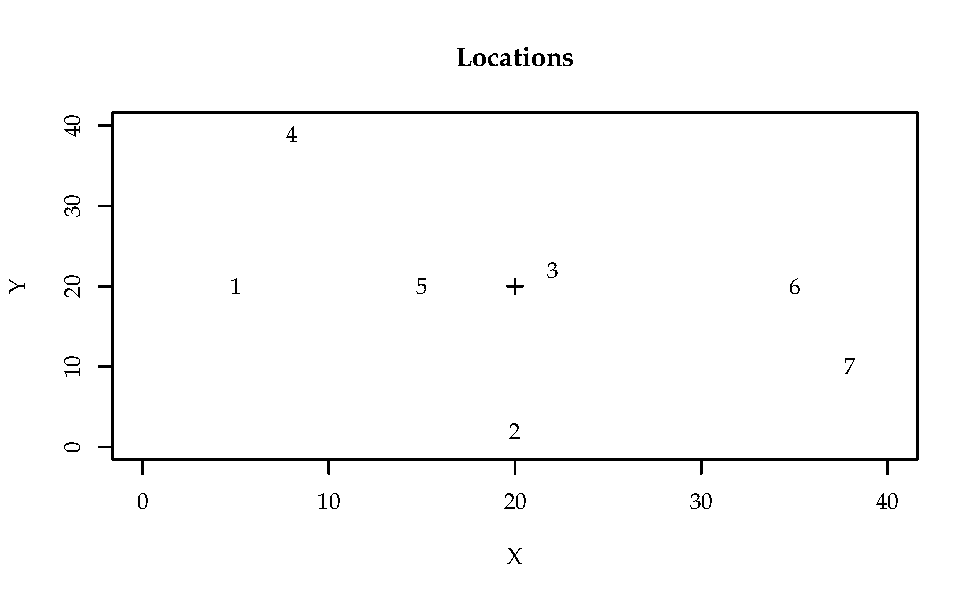
\includegraphics[width=\maxwidth]{figure/prob1x-1} 

}



\end{knitrout}

\newpage

\begin{enumerate}
\item %1a
{\it Do the same conclusions regarding the effects of the sill, range, and nugget effect still hold?}

Yes, the effects still hold.

{\bf Effect of Sill}

The relative sill, range, and nugget parameters are the same with the model with the two locations changed as with the original model. 

Model A and Model E both have a practical range of 20 and nugget of 0, with an exponential covariance model. Model A has half the sill of model E. Yes, the effects on predicts and kriging variance stay the same as before. The predictions ad weights are the same with Models A and E and the kriging variance of Model E is twice the kriging variance of Model A, as with the original locations.

{\bf Effect of (Practical) Range}

Models A and B both have nugget effects of 0 and sills of 10 with an exponential specified covariance model. The (practial) range is 20 for Model A and 10 for Model B. The predictions, kriging variance, and weights are all different between the two models, but again have similar effects as those in the original model. Model B assigns more weight to locations farther away from the prediction location and less weight to locations closer to the prediction location than Model A does. This makes sense because specifying a larger practical range takes more information from points farther away. Likewise, again we see the kriging variance increase for Model B where there is a larger practical range.

{\bf Effect of Nugget}

Models A and C both have ranges of 20 and sills of 10. The nugget for Model A is 0 while the nugget for Model C is 5. Model D is a pure nugget model. The weights and predicions the same between the two models. The variance without a nugget effect is twice the variance with the nugget effect because with a sill of 10 in both and a nugget of 5, half the total variation is absorbed by the nugget, removing half the variation that could be attributed to spatial correlations. These conclusions are again the same as with the original data. We see the pure nugget model (Model D) differs from both Model A and Model B in predictions, kriging variance, and weights. With a pure nugget effect, all locations have equal weights and the variance is much larger.



\item 
{\it Which points are screening?}

Points 3 and 5 are screening as they have larger weights and are at closer distances.

\item

{\it What happens to the kriging variance?}

The kriging variance is smallest with the gaussian model, although the gaussian model does return negative weights.

The kriging variance decreases in the presence of a nugget, increases with a decrease in practical range (less information), increases with an increased sill, and in the absence of spatial correlation is very close to the nugget.

\item
{\it In which models does the predicted value change and in which does it stay the same?}

Models A, C and E all predicted the same value. These models all had the same practical range and were fit with the exponential model.

Models B, D, and F all had different predicted values. Models D and F were fit with different models (nugget and gaussian, respectfully) and Model B had half the practical range as models A, C, and E.

\end{enumerate}

\item
{\it We are going to use ordinary kriging to predict values of total carbon over a grid. You should still have the carbon/nitrogen data set from the last homework but let me know if you need to have it emailed to you. Choose your grid to be the same as in the CN ratio example I worked in class. Set up R code is below.}



{\it We will work with total carbon (column labelled TC in the data set) in this problem. You can use either the ksline or krige.conv functions. Be a bit patient; it should take only a minute or so. Don’t worry about anisotropy.}
\begin{enumerate}
\item {\it Plot the data. Do you see any evidence of trend? Outliers? Other potential anomalies?}

The data appear to be grided. Trends do not appear in either the north-south nor the east-west directions. Trying very hard to make a trend, you might say there's a very slight negative linear trend in the north-south direction. A few outliers stand out appear in both vertical and horizontal directions. The shapes (colors) which represent the quartiles in the top left plot appear to mostly occur in clusteres. This means that data in similar quantiles appear to be located closer together. The data are normally distributed, with a very minimal left skew.

\begin{knitrout}\footnotesize
\definecolor{shadecolor}{rgb}{0.969, 0.969, 0.969}\color{fgcolor}

{\centering 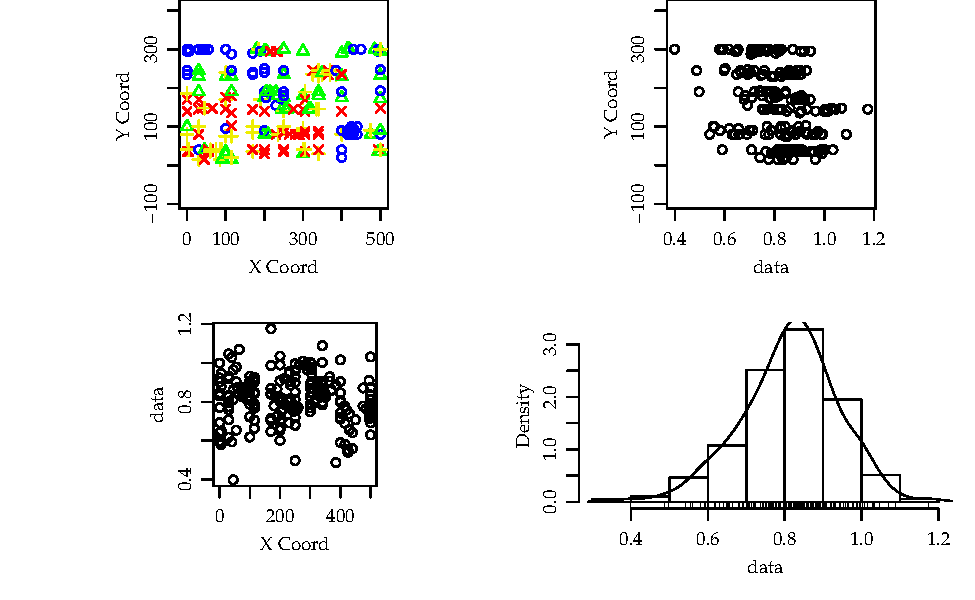
\includegraphics[width=\maxwidth]{figure/prob2a-1} 

}



\end{knitrout}

\item 
{\it Predict using global ordinary kriging. You estimated a semivariogram for these data on the last homework and you can use those results. Prepare contour plots of the predictions and kriging standard errors.}

\begin{knitrout}\footnotesize
\definecolor{shadecolor}{rgb}{0.969, 0.969, 0.969}\color{fgcolor}\begin{kframe}
\begin{verbatim}
variog: computing omnidirectional variogram
variofit: covariance model used is exponential 
variofit: weights used: equal 
variofit: minimisation function used: optim 
\end{verbatim}
\end{kframe}

{\centering 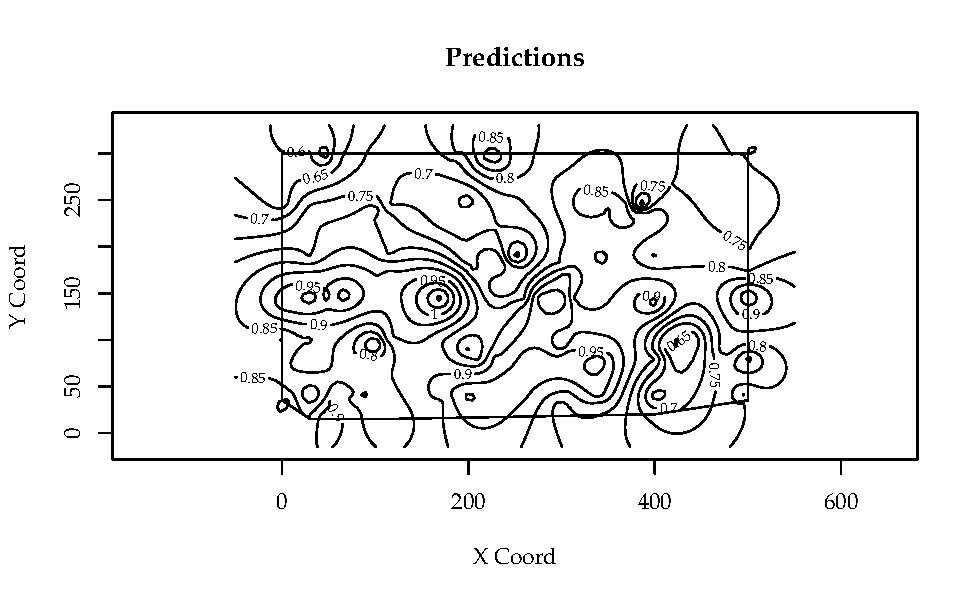
\includegraphics[width=\maxwidth]{figure/prob2b-1} 

}




{\centering 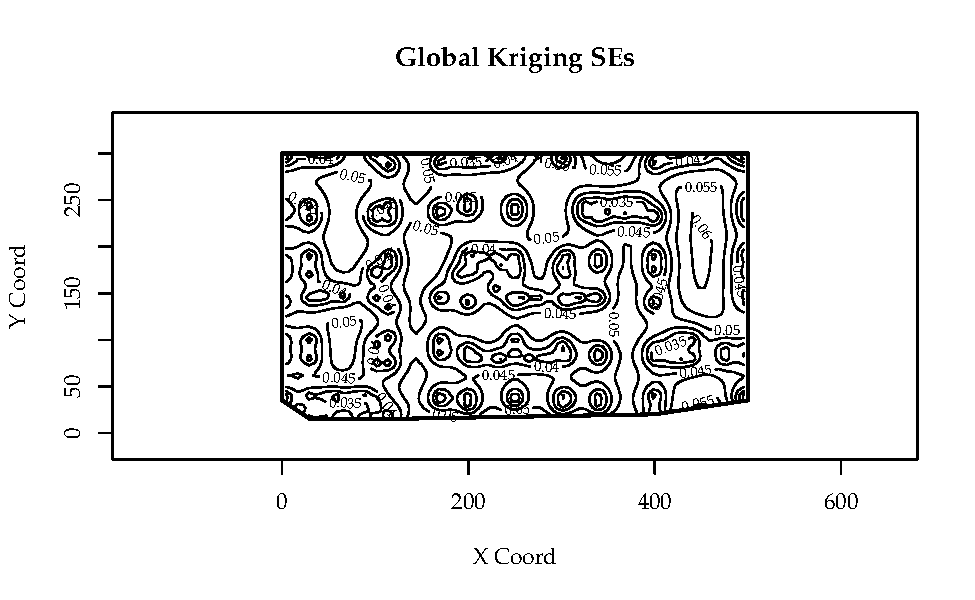
\includegraphics[width=\maxwidth]{figure/prob2b-2} 

}



\end{knitrout}

\item
{\it Evaluate the predictions using cross validation (CV2). You can use the R code I provided in class notes.}

I also computed CV1, which is quite closer to 0, than CV2 is to 1. 

Having CV2 close to 1 means that the sqrt(MSEP) is unbiased for the kriging variance among all j location removals. CV2 is above 1, meaning that the sqrt(MSEP) is a biased measure for the kriging variance. The predictions are off more than expected.



% latex table generated in R 3.3.2 by xtable 1.8-2 package
% Fri Feb 24 11:36:08 2017
\begin{table}[ht]
\centering
\begin{tabular}{|l|l||}
  \hline
CV1 & CV2 \\ 
  \hline
0.01 & 1.53 \\ 
   \hline
\end{tabular}
\end{table}


\item {Briefly discuss your results.}

The prediction plot shows quite a few contours with step slopes, and so is not that smooth. The global kriging SE's were all not very large, but also have quite a few steep controus. Prediction at locations with steep contours will change rapidly even when the SE's are not very large, but may explain some of the bias suggested by the CV2 value.

We do see the lowest predictions are in the upper left and lower right corners, as was suggested by the colored plot of the original data where the clusers with the lowest quantile are at.

In part 
\end{enumerate}

\end{enumerate}

\section*{R Code}

{\bf Problem 1}

\begin{knitrout}\footnotesize
\definecolor{shadecolor}{rgb}{0.969, 0.969, 0.969}\color{fgcolor}\begin{kframe}
\begin{alltt}
\hlstd{x} \hlkwb{<-} \hlkwd{c}\hlstd{(}\hlnum{5}\hlstd{,}\hlnum{20}\hlstd{,}\hlnum{25}\hlstd{,}\hlnum{8}\hlstd{,}\hlnum{10}\hlstd{,}\hlnum{35}\hlstd{,}\hlnum{38}\hlstd{)}
\hlstd{y} \hlkwb{<-} \hlkwd{c}\hlstd{(}\hlnum{20}\hlstd{,}\hlnum{2}\hlstd{,}\hlnum{32}\hlstd{,}\hlnum{39}\hlstd{,}\hlnum{17}\hlstd{,}\hlnum{20}\hlstd{,}\hlnum{10}\hlstd{)}
\hlstd{z} \hlkwb{<-} \hlkwd{c}\hlstd{(}\hlnum{100}\hlstd{,}\hlnum{70}\hlstd{,}\hlnum{60}\hlstd{,}\hlnum{90}\hlstd{,}\hlnum{50}\hlstd{,}\hlnum{80}\hlstd{,}\hlnum{40}\hlstd{)}

\hlstd{loc} \hlkwb{<-} \hlkwd{data.frame}\hlstd{(}\hlkwd{cbind}\hlstd{(x,y,z))}
\hlkwd{colnames}\hlstd{(loc)} \hlkwb{<-} \hlkwd{c}\hlstd{(}\hlstr{"x"}\hlstd{,} \hlstr{"y"}\hlstd{,} \hlstr{"z"}\hlstd{)}

\hlstd{loc.new} \hlkwb{<-} \hlstd{loc}
\hlstd{loc.new[}\hlnum{3}\hlstd{,}\hlkwd{c}\hlstd{(}\hlnum{1}\hlstd{,}\hlnum{2}\hlstd{)]} \hlkwb{<-} \hlkwd{c}\hlstd{(}\hlnum{22}\hlstd{,}\hlnum{22}\hlstd{)}
\hlstd{loc.new[}\hlnum{5}\hlstd{,}\hlkwd{c}\hlstd{(}\hlnum{1}\hlstd{,}\hlnum{2}\hlstd{)]} \hlkwb{<-} \hlkwd{c}\hlstd{(}\hlnum{15}\hlstd{,}\hlnum{20}\hlstd{)}

\hlstd{dist.new} \hlkwb{<-} \hlkwd{as.matrix}\hlstd{(}\hlkwd{dist}\hlstd{(loc.new[,}\hlnum{1}\hlopt{:}\hlnum{2}\hlstd{]))}

\hlstd{sigma.vec.new} \hlkwb{<-} \hlkwd{as.matrix}\hlstd{(}\hlkwd{dist}\hlstd{(}\hlkwd{rbind}\hlstd{(loc.new[,}\hlnum{1}\hlopt{:}\hlnum{2}\hlstd{],}\hlkwd{c}\hlstd{(}\hlnum{20}\hlstd{,}\hlnum{20}\hlstd{))))}
\hlstd{sigma.vec.new} \hlkwb{<-} \hlstd{sigma.vec.new[}\hlnum{8}\hlstd{,]}
\hlstd{sigma.vec.new[}\hlnum{8}\hlstd{]} \hlkwb{<-} \hlnum{1}

\hlstd{sigma.vec.old} \hlkwb{<-} \hlkwd{as.matrix}\hlstd{(}\hlkwd{dist}\hlstd{(}\hlkwd{rbind}\hlstd{(loc[,}\hlnum{1}\hlopt{:}\hlnum{2}\hlstd{],}\hlkwd{c}\hlstd{(}\hlnum{20}\hlstd{,}\hlnum{20}\hlstd{))))}
\hlstd{sigma.vec.old} \hlkwb{<-} \hlstd{sigma.vec.old[}\hlnum{8}\hlstd{,]}
\hlstd{sigma.vec.old[}\hlnum{8}\hlstd{]} \hlkwb{<-} \hlnum{1}
\end{alltt}
\end{kframe}
\end{knitrout}
\begin{knitrout}\footnotesize
\definecolor{shadecolor}{rgb}{0.969, 0.969, 0.969}\color{fgcolor}\begin{kframe}
\begin{alltt}
\hlstd{x} \hlkwb{<-} \hlkwd{c}\hlstd{(}\hlnum{5}\hlstd{,}\hlnum{20}\hlstd{,}\hlnum{25}\hlstd{,}\hlnum{8}\hlstd{,}\hlnum{10}\hlstd{,}\hlnum{35}\hlstd{,}\hlnum{38}\hlstd{)}
\hlstd{y} \hlkwb{<-} \hlkwd{c}\hlstd{(}\hlnum{20}\hlstd{,}\hlnum{2}\hlstd{,}\hlnum{32}\hlstd{,}\hlnum{39}\hlstd{,}\hlnum{17}\hlstd{,}\hlnum{20}\hlstd{,}\hlnum{10}\hlstd{)}
\hlstd{z} \hlkwb{<-} \hlkwd{c}\hlstd{(}\hlnum{100}\hlstd{,}\hlnum{70}\hlstd{,}\hlnum{60}\hlstd{,}\hlnum{90}\hlstd{,}\hlnum{50}\hlstd{,}\hlnum{80}\hlstd{,}\hlnum{40}\hlstd{)}

\hlstd{loc} \hlkwb{<-} \hlkwd{data.frame}\hlstd{(}\hlkwd{cbind}\hlstd{(x,y,z))}
\hlkwd{colnames}\hlstd{(loc)} \hlkwb{<-} \hlkwd{c}\hlstd{(}\hlstr{"x"}\hlstd{,} \hlstr{"y"}\hlstd{,} \hlstr{"z"}\hlstd{)}

\hlstd{loc.new} \hlkwb{<-} \hlstd{loc}
\hlstd{loc.new[}\hlnum{3}\hlstd{,}\hlkwd{c}\hlstd{(}\hlnum{1}\hlstd{,}\hlnum{2}\hlstd{)]} \hlkwb{<-} \hlkwd{c}\hlstd{(}\hlnum{22}\hlstd{,}\hlnum{22}\hlstd{)}
\hlstd{loc.new[}\hlnum{5}\hlstd{,}\hlkwd{c}\hlstd{(}\hlnum{1}\hlstd{,}\hlnum{2}\hlstd{)]} \hlkwb{<-} \hlkwd{c}\hlstd{(}\hlnum{15}\hlstd{,}\hlnum{20}\hlstd{)}

\hlstd{dist.new} \hlkwb{<-} \hlkwd{as.matrix}\hlstd{(}\hlkwd{dist}\hlstd{(loc.new[,}\hlnum{1}\hlopt{:}\hlnum{2}\hlstd{]))}

\hlstd{sigma.vec.new} \hlkwb{<-} \hlkwd{as.matrix}\hlstd{(}\hlkwd{dist}\hlstd{(}\hlkwd{rbind}\hlstd{(loc.new[,}\hlnum{1}\hlopt{:}\hlnum{2}\hlstd{],}\hlkwd{c}\hlstd{(}\hlnum{20}\hlstd{,}\hlnum{20}\hlstd{))))}
\hlstd{sigma.vec.new} \hlkwb{<-} \hlstd{sigma.vec.new[}\hlnum{8}\hlstd{,]}
\hlstd{sigma.vec.new[}\hlnum{8}\hlstd{]} \hlkwb{<-} \hlnum{1}

\hlstd{sigma.vec.old} \hlkwb{<-} \hlkwd{as.matrix}\hlstd{(}\hlkwd{dist}\hlstd{(}\hlkwd{rbind}\hlstd{(loc[,}\hlnum{1}\hlopt{:}\hlnum{2}\hlstd{],}\hlkwd{c}\hlstd{(}\hlnum{20}\hlstd{,}\hlnum{20}\hlstd{))))}
\hlstd{sigma.vec.old} \hlkwb{<-} \hlstd{sigma.vec.old[}\hlnum{8}\hlstd{,]}
\hlstd{sigma.vec.old[}\hlnum{8}\hlstd{]} \hlkwb{<-} \hlnum{1}

\hlstd{dist.old} \hlkwb{<-} \hlkwd{as.matrix}\hlstd{(}\hlkwd{dist}\hlstd{(loc[,}\hlnum{1}\hlopt{:}\hlnum{2}\hlstd{]))}
\hlstd{sigma.vec} \hlkwb{<-} \hlkwd{as.matrix}\hlstd{(}\hlkwd{dist}\hlstd{(}\hlkwd{rbind}\hlstd{(loc[,}\hlnum{1}\hlopt{:}\hlnum{2}\hlstd{],}\hlkwd{c}\hlstd{(}\hlnum{20}\hlstd{,}\hlnum{20}\hlstd{))))}
\hlstd{sigma.vec} \hlkwb{<-} \hlstd{sigma.vec[}\hlnum{8}\hlstd{,]}
\hlstd{sigma.vec[}\hlnum{8}\hlstd{]} \hlkwb{<-} \hlnum{1}


\hlcom{# try to automate}
\hlstd{dmat.old} \hlkwb{<-} \hlkwd{as.matrix}\hlstd{(dist.old)}
\hlstd{dmat.new} \hlkwb{<-} \hlkwd{as.matrix}\hlstd{(dist.new)}

\hlstd{sig.fn} \hlkwb{<-} \hlkwa{function}\hlstd{(}\hlkwc{dmat}\hlstd{,} \hlkwc{model}\hlstd{,} \hlkwc{sill}\hlstd{,} \hlkwc{nugget}\hlstd{,} \hlkwc{range}\hlstd{,} \hlkwc{offset}\hlstd{,} \hlkwc{sigma.vec}\hlstd{,} \hlkwc{location}\hlstd{)\{}
  \hlstd{Sigma} \hlkwb{<-} \hlkwd{cov.spatial}\hlstd{(dmat,} \hlkwc{cov.model} \hlstd{= model,}
                       \hlkwc{cov.pars}\hlstd{=}\hlkwd{c}\hlstd{(sill} \hlopt{-} \hlstd{nugget, range}\hlopt{/}\hlstd{offset))}
  \hlstd{pred} \hlkwb{<-} \hlkwd{c}\hlstd{(}\hlkwd{rep}\hlstd{(}\hlnum{1}\hlstd{,}\hlnum{7}\hlstd{))}
\hlstd{Sigma.star} \hlkwb{<-} \hlkwd{data.frame}\hlstd{(}\hlkwd{cbind}\hlstd{(Sigma,pred))}
\hlstd{pred} \hlkwb{<-} \hlkwd{c}\hlstd{(}\hlkwd{rep}\hlstd{(}\hlnum{1}\hlstd{,}\hlnum{7}\hlstd{),}\hlnum{0}\hlstd{)}
\hlstd{Sigma.star[}\hlnum{8}\hlstd{,]} \hlkwb{<-} \hlkwd{c}\hlstd{(pred)}

\hlcom{# find sigma star}
\hlstd{sigma.star} \hlkwb{<-} \hlkwd{cov.spatial}\hlstd{(sigma.vec,}\hlkwc{cov.model}\hlstd{=model,} \hlkwc{cov.pars}\hlstd{=}\hlkwd{c}\hlstd{((sill} \hlopt{-} \hlstd{nugget), range}\hlopt{/}\hlstd{offset))}
\hlstd{sigma.star[}\hlnum{8}\hlstd{]} \hlkwb{<-} \hlnum{1}
\hlstd{sigma.star} \hlkwb{<-} \hlkwd{t}\hlstd{(}\hlkwd{as.matrix}\hlstd{(sigma.star))}

\hlstd{lambda.star} \hlkwb{<-} \hlstd{sigma.star} \hlopt \hlkwd{solve}\hlstd{(Sigma.star)}

\hlstd{pred.new} \hlkwb{<-} \hlkwd{sum}\hlstd{(lambda.star[}\hlopt{-}\hlnum{8}\hlstd{]}\hlopt{*}\hlstd{location[,}\hlnum{3}\hlstd{])}
\hlstd{var.new} \hlkwb{<-} \hlstd{sill} \hlopt{-} \hlstd{nugget} \hlopt{-} \hlkwd{sum}\hlstd{(lambda.star}\hlopt{*}\hlstd{sigma.star)}

\hlkwd{return}\hlstd{(}\hlkwd{c}\hlstd{(pred.new, var.new,} \hlkwd{c}\hlstd{(lambda.star)[}\hlopt{-}\hlnum{8}\hlstd{]))}
\hlstd{\}}

\hlcom{# dmat, model, sill, nugget, range, offset, sigma.vec, location}

\hlstd{A.old} \hlkwb{<-} \hlkwd{sig.fn}\hlstd{(}\hlkwc{dmat} \hlstd{= dist.old,} \hlkwc{sill} \hlstd{=} \hlnum{10}\hlstd{,}
                \hlkwc{nugget} \hlstd{=} \hlnum{0}\hlstd{,} \hlkwc{range} \hlstd{=} \hlnum{20}\hlstd{,} \hlkwc{offset} \hlstd{=} \hlnum{3}\hlstd{,}
                \hlkwc{model} \hlstd{=} \hlstr{"exponential"}\hlstd{,}
                \hlkwc{sigma.vec} \hlstd{= sigma.vec.old,}
                \hlkwc{location} \hlstd{= loc)}

\hlstd{B.old} \hlkwb{<-} \hlkwd{sig.fn}\hlstd{(}\hlkwc{dmat} \hlstd{= dist.old,} \hlkwc{sill} \hlstd{=} \hlnum{10}\hlstd{,}
                \hlkwc{nugget} \hlstd{=} \hlnum{0}\hlstd{,} \hlkwc{range} \hlstd{=} \hlnum{10}\hlstd{,} \hlkwc{offset} \hlstd{=} \hlnum{3}\hlstd{,}
                \hlkwc{model} \hlstd{=} \hlstr{"exponential"}\hlstd{,}
                \hlkwc{sigma.vec} \hlstd{= sigma.vec.old,}
                \hlkwc{location} \hlstd{= loc)}

\hlstd{C.old} \hlkwb{<-} \hlkwd{sig.fn}\hlstd{(}\hlkwc{dmat} \hlstd{= dist.old,} \hlkwc{sill} \hlstd{=} \hlnum{10}\hlstd{,}
                \hlkwc{nugget} \hlstd{=} \hlnum{5}\hlstd{,} \hlkwc{range} \hlstd{=} \hlnum{20}\hlstd{,} \hlkwc{offset} \hlstd{=} \hlnum{3}\hlstd{,}
                \hlkwc{model} \hlstd{=} \hlstr{"exponential"}\hlstd{,}
                \hlkwc{sigma.vec} \hlstd{= sigma.vec.old,}
                \hlkwc{location} \hlstd{= loc)}

\hlstd{Sigma.oldD} \hlkwb{<-} \hlkwd{diag}\hlstd{(}\hlnum{5}\hlstd{,}\hlnum{7}\hlstd{,}\hlnum{7}\hlstd{)}
\hlstd{pred} \hlkwb{<-} \hlkwd{c}\hlstd{(}\hlkwd{rep}\hlstd{(}\hlnum{1}\hlstd{,}\hlnum{7}\hlstd{))}
\hlstd{Sigma.star.oldD} \hlkwb{<-} \hlkwd{data.frame}\hlstd{(}\hlkwd{cbind}\hlstd{(Sigma.oldD,pred))}
\hlstd{pred} \hlkwb{<-} \hlkwd{c}\hlstd{(}\hlkwd{rep}\hlstd{(}\hlnum{1}\hlstd{,}\hlnum{7}\hlstd{),}\hlnum{0}\hlstd{)}
\hlstd{Sigma.star.oldD[}\hlnum{8}\hlstd{,]} \hlkwb{<-} \hlkwd{c}\hlstd{(pred)}

\hlcom{# find sigma star}
\hlstd{sigma.star.oldD} \hlkwb{<-} \hlkwd{c}\hlstd{(}\hlkwd{rep}\hlstd{(}\hlnum{0}\hlstd{,}\hlnum{7}\hlstd{),}\hlnum{1}\hlstd{)}
\hlstd{sigma.star.oldD} \hlkwb{<-} \hlkwd{t}\hlstd{(}\hlkwd{as.matrix}\hlstd{(sigma.star.oldD))}

\hlstd{lambda.star.oldD} \hlkwb{<-} \hlstd{sigma.star.oldD} \hlopt \hlkwd{solve}\hlstd{(Sigma.star.oldD)}

\hlstd{pred.oldD} \hlkwb{<-} \hlkwd{sum}\hlstd{(lambda.star.oldD[}\hlopt{-}\hlnum{8}\hlstd{]}\hlopt{*}\hlstd{loc[,}\hlnum{3}\hlstd{])}
\hlstd{var.oldD} \hlkwb{<-} \hlnum{10}\hlopt{-}\hlkwd{sum}\hlstd{(lambda.star.oldD}\hlopt{*}\hlstd{sigma.star.oldD)}

\hlstd{D.old} \hlkwb{<-} \hlkwd{c}\hlstd{(pred.oldD, var.oldD,}
           \hlkwd{c}\hlstd{(lambda.star.oldD[}\hlopt{-}\hlnum{8}\hlstd{]))}

\hlstd{E.old} \hlkwb{<-} \hlkwd{sig.fn}\hlstd{(}\hlkwc{dmat} \hlstd{= dist.old,} \hlkwc{sill} \hlstd{=} \hlnum{20}\hlstd{,}
                \hlkwc{nugget} \hlstd{=} \hlnum{0}\hlstd{,} \hlkwc{range} \hlstd{=} \hlnum{20}\hlstd{,} \hlkwc{offset} \hlstd{=} \hlnum{3}\hlstd{,}
                \hlkwc{model} \hlstd{=} \hlstr{"exponential"}\hlstd{,}
                \hlkwc{sigma.vec} \hlstd{= sigma.vec.old,}
                \hlkwc{location} \hlstd{= loc)}

\hlstd{F.old} \hlkwb{<-} \hlkwd{sig.fn}\hlstd{(}\hlkwc{dmat} \hlstd{= dist.old,} \hlkwc{sill} \hlstd{=} \hlnum{10}\hlstd{,}
                \hlkwc{nugget} \hlstd{=} \hlnum{0}\hlstd{,} \hlkwc{range} \hlstd{=} \hlnum{20}\hlstd{,} \hlkwc{offset} \hlstd{=} \hlkwd{sqrt}\hlstd{(}\hlnum{3}\hlstd{),}
                \hlkwc{model} \hlstd{=} \hlstr{"gaussian"}\hlstd{,}
                \hlkwc{sigma.vec} \hlstd{= sigma.vec.old,}
                \hlkwc{location} \hlstd{= loc)}

\hlstd{dist.old.out} \hlkwb{<-} \hlkwd{as.matrix}\hlstd{(}\hlkwd{dist}\hlstd{(}\hlkwd{data.frame}\hlstd{(}\hlkwd{rbind}\hlstd{(loc[,}\hlnum{1}\hlopt{:}\hlnum{2}\hlstd{],}\hlkwd{c}\hlstd{(}\hlnum{20}\hlstd{,}\hlnum{20}\hlstd{)))))[}\hlnum{8}\hlstd{,}\hlopt{-}\hlnum{8}\hlstd{]}

\hlstd{old} \hlkwb{<-} \hlkwd{data.frame}\hlstd{(}\hlkwd{rbind}\hlstd{(A.old, B.old, C.old, D.old, E.old,}
                        \hlstd{F.old,} \hlkwd{c}\hlstd{(}\hlstr{""}\hlstd{,} \hlstr{""}\hlstd{, dist.old.out)))}
\hlkwd{colnames}\hlstd{(old)} \hlkwb{<-} \hlkwd{c}\hlstd{(}\hlstr{"rho.pred"}\hlstd{,} \hlstr{"sigma2.pred"}\hlstd{,} \hlstr{"lambda1"}\hlstd{,} \hlstr{"lambda2"}\hlstd{,} \hlstr{"lambda3"}\hlstd{,}
                      \hlstr{"lambda4"}\hlstd{,} \hlstr{"lambda5"}\hlstd{,} \hlstr{"lambda6"}\hlstd{,} \hlstr{"lambda7"}\hlstd{)}

\hlstd{a} \hlkwb{<-} \hlkwd{rownames}\hlstd{(old)}

\hlstd{old} \hlkwb{<-} \hlkwd{data.frame}\hlstd{(}\hlkwd{apply}\hlstd{(old,} \hlnum{2}\hlstd{,} \hlkwa{function}\hlstd{(}\hlkwc{t}\hlstd{)\{}
  \hlkwd{round}\hlstd{(}\hlkwd{as.numeric}\hlstd{(t),}\hlnum{2}\hlstd{)}
\hlstd{\}))}

\hlkwd{rownames}\hlstd{(old)} \hlkwb{<-} \hlkwd{c}\hlstd{(a)}

\hlkwd{print}\hlstd{(}\hlkwd{xtable}\hlstd{(old,} \hlkwc{align} \hlstd{=} \hlstr{"||l|l|l|l|l|l|l|l|l|l||"}\hlstd{))}

\hlstd{A.new} \hlkwb{<-} \hlkwd{sig.fn}\hlstd{(}\hlkwc{dmat} \hlstd{= dist.new,} \hlkwc{sill} \hlstd{=} \hlnum{10}\hlstd{,}
                \hlkwc{nugget} \hlstd{=} \hlnum{0}\hlstd{,} \hlkwc{range} \hlstd{=} \hlnum{20}\hlstd{,} \hlkwc{offset} \hlstd{=} \hlnum{3}\hlstd{,}
                \hlkwc{model} \hlstd{=} \hlstr{"exponential"}\hlstd{,}
                \hlkwc{sigma.vec} \hlstd{= sigma.vec.new,}
                \hlkwc{location} \hlstd{= loc.new)}

\hlstd{B.new} \hlkwb{<-} \hlkwd{sig.fn}\hlstd{(}\hlkwc{dmat} \hlstd{= dist.new,} \hlkwc{sill} \hlstd{=} \hlnum{10}\hlstd{,}
                \hlkwc{nugget} \hlstd{=} \hlnum{0}\hlstd{,} \hlkwc{range} \hlstd{=} \hlnum{10}\hlstd{,} \hlkwc{offset} \hlstd{=} \hlnum{3}\hlstd{,}
                \hlkwc{model} \hlstd{=} \hlstr{"exponential"}\hlstd{,}
                \hlkwc{sigma.vec} \hlstd{= sigma.vec.new,}
                \hlkwc{location} \hlstd{= loc.new)}

\hlstd{C.new} \hlkwb{<-} \hlkwd{sig.fn}\hlstd{(}\hlkwc{dmat} \hlstd{= dist.new,} \hlkwc{sill} \hlstd{=} \hlnum{10}\hlstd{,}
                \hlkwc{nugget} \hlstd{=} \hlnum{5}\hlstd{,} \hlkwc{range} \hlstd{=} \hlnum{20}\hlstd{,} \hlkwc{offset} \hlstd{=} \hlnum{3}\hlstd{,}
                \hlkwc{model} \hlstd{=} \hlstr{"exponential"}\hlstd{,}
                \hlkwc{sigma.vec} \hlstd{= sigma.vec.new,}
                \hlkwc{location} \hlstd{= loc.new)}

\hlstd{Sigma.newD} \hlkwb{<-} \hlkwd{diag}\hlstd{(}\hlnum{5}\hlstd{,}\hlnum{7}\hlstd{,}\hlnum{7}\hlstd{)}
\hlstd{pred} \hlkwb{<-} \hlkwd{c}\hlstd{(}\hlkwd{rep}\hlstd{(}\hlnum{1}\hlstd{,}\hlnum{7}\hlstd{))}
\hlstd{Sigma.star.newD} \hlkwb{<-} \hlkwd{data.frame}\hlstd{(}\hlkwd{cbind}\hlstd{(Sigma.newD,pred))}
\hlstd{pred} \hlkwb{<-} \hlkwd{c}\hlstd{(}\hlkwd{rep}\hlstd{(}\hlnum{1}\hlstd{,}\hlnum{7}\hlstd{),}\hlnum{0}\hlstd{)}
\hlstd{Sigma.star.newD[}\hlnum{8}\hlstd{,]} \hlkwb{<-} \hlkwd{c}\hlstd{(pred)}

\hlcom{# find sigma star}
\hlstd{sigma.star.newD} \hlkwb{<-} \hlkwd{c}\hlstd{(}\hlkwd{rep}\hlstd{(}\hlnum{0}\hlstd{,}\hlnum{7}\hlstd{),}\hlnum{1}\hlstd{)}
\hlstd{sigma.star.newD} \hlkwb{<-} \hlkwd{t}\hlstd{(}\hlkwd{as.matrix}\hlstd{(sigma.star.newD))}

\hlstd{lambda.star.newD} \hlkwb{<-} \hlstd{sigma.star.newD} \hlopt \hlkwd{solve}\hlstd{(Sigma.star.newD)}

\hlstd{pred.newD} \hlkwb{<-} \hlkwd{sum}\hlstd{(lambda.star.newD[}\hlopt{-}\hlnum{8}\hlstd{]}\hlopt{*}\hlstd{loc.new[,}\hlnum{3}\hlstd{])}
\hlstd{var.newD} \hlkwb{<-} \hlnum{10}\hlopt{-}\hlkwd{sum}\hlstd{(lambda.star.newD}\hlopt{*}\hlstd{sigma.star.newD)}

\hlstd{D.new} \hlkwb{<-} \hlkwd{c}\hlstd{(pred.newD, var.newD,}
           \hlkwd{c}\hlstd{(lambda.star.newD[}\hlopt{-}\hlnum{8}\hlstd{]))}


\hlstd{E.new} \hlkwb{<-} \hlkwd{sig.fn}\hlstd{(}\hlkwc{dmat} \hlstd{= dist.new,} \hlkwc{sill} \hlstd{=} \hlnum{20}\hlstd{,}
                \hlkwc{nugget} \hlstd{=} \hlnum{0}\hlstd{,} \hlkwc{range} \hlstd{=} \hlnum{20}\hlstd{,} \hlkwc{offset} \hlstd{=} \hlnum{3}\hlstd{,}
                \hlkwc{model} \hlstd{=} \hlstr{"exponential"}\hlstd{,}
                \hlkwc{sigma.vec} \hlstd{= sigma.vec.new,}
                \hlkwc{location} \hlstd{= loc.new)}

\hlstd{F.new} \hlkwb{<-} \hlkwd{sig.fn}\hlstd{(}\hlkwc{dmat} \hlstd{= dist.new,} \hlkwc{sill} \hlstd{=} \hlnum{10}\hlstd{,}
                \hlkwc{nugget} \hlstd{=} \hlnum{0}\hlstd{,} \hlkwc{range} \hlstd{=} \hlnum{20}\hlstd{,} \hlkwc{offset} \hlstd{=} \hlkwd{sqrt}\hlstd{(}\hlnum{3}\hlstd{),}
                \hlkwc{model} \hlstd{=} \hlstr{"gaussian"}\hlstd{,}
                \hlkwc{sigma.vec} \hlstd{= sigma.vec.new,}
                \hlkwc{location} \hlstd{= loc.new)}

\hlstd{dist.new.out} \hlkwb{<-} \hlkwd{as.matrix}\hlstd{(}\hlkwd{dist}\hlstd{(}\hlkwd{data.frame}\hlstd{(}\hlkwd{rbind}\hlstd{(loc.new[,}\hlnum{1}\hlopt{:}\hlnum{2}\hlstd{],}\hlkwd{c}\hlstd{(}\hlnum{20}\hlstd{,}\hlnum{20}\hlstd{)))))[}\hlnum{8}\hlstd{,}\hlopt{-}\hlnum{8}\hlstd{]}

\hlstd{new.out} \hlkwb{<-} \hlkwd{data.frame}\hlstd{(}\hlkwd{rbind}\hlstd{(A.new, B.new, C.new, D.new, E.new,F.new,}\hlkwd{c}\hlstd{(}\hlstr{""}\hlstd{,} \hlstr{""}\hlstd{, dist.new.out)))}
\hlkwd{colnames}\hlstd{(new.out)} \hlkwb{<-}  \hlkwd{c}\hlstd{(}\hlstr{"rho.pred"}\hlstd{,} \hlstr{"sigma2.pred"}\hlstd{,} \hlstr{"lambda1"}\hlstd{,} \hlstr{"lambda2"}\hlstd{,} \hlstr{"lambda3"}\hlstd{,}
                      \hlstr{"lambda4"}\hlstd{,} \hlstr{"lambda5"}\hlstd{,} \hlstr{"lambda6"}\hlstd{,} \hlstr{"lambda7"}\hlstd{)}

\hlstd{b} \hlkwb{<-} \hlkwd{rownames}\hlstd{(new.out)}

\hlstd{new.out} \hlkwb{<-} \hlkwd{data.frame}\hlstd{(}\hlkwd{apply}\hlstd{(new.out,} \hlnum{2}\hlstd{,} \hlkwa{function}\hlstd{(}\hlkwc{t}\hlstd{)\{}
  \hlkwd{round}\hlstd{(}\hlkwd{as.numeric}\hlstd{(t),}\hlnum{2}\hlstd{)}
\hlstd{\}))}

\hlkwd{rownames}\hlstd{(new.out)} \hlkwb{<-} \hlkwd{c}\hlstd{(b)}


\hlkwd{print}\hlstd{(}\hlkwd{xtable}\hlstd{(new.out,} \hlkwc{align} \hlstd{=} \hlstr{"||l|l|l|l|l|l|l|l|l|l||"}\hlstd{))}
\end{alltt}
\end{kframe}
\end{knitrout}
\begin{knitrout}\footnotesize
\definecolor{shadecolor}{rgb}{0.969, 0.969, 0.969}\color{fgcolor}\begin{kframe}
\begin{alltt}
\hlstd{names} \hlkwb{<-} \hlkwd{c}\hlstd{(}\hlstr{"1"}\hlstd{,} \hlstr{"2"}\hlstd{,} \hlstr{"3"}\hlstd{,} \hlstr{"4"}\hlstd{,} \hlstr{"5"}\hlstd{,} \hlstr{"6"}\hlstd{,} \hlstr{"7"}\hlstd{)}
\hlkwd{plot}\hlstd{(}\hlkwc{x}\hlstd{=loc.new}\hlopt{$}\hlstd{x,}\hlkwc{y}\hlstd{=loc.new}\hlopt{$}\hlstd{y,} \hlkwc{pch}\hlstd{=names,} \hlkwc{xlim} \hlstd{=} \hlkwd{c}\hlstd{(}\hlnum{0}\hlstd{,}\hlnum{40}\hlstd{),} \hlkwc{ylim}\hlstd{=}\hlkwd{c}\hlstd{(}\hlnum{0}\hlstd{,}\hlnum{40}\hlstd{),} \hlkwc{main} \hlstd{=} \hlstr{"Locations"}\hlstd{,}
     \hlkwc{xlab} \hlstd{=} \hlstr{"X"}\hlstd{,} \hlkwc{ylab} \hlstd{=} \hlstr{"Y"}\hlstd{)}
\hlkwd{points}\hlstd{(}\hlnum{20}\hlstd{,}\hlnum{20}\hlstd{,}\hlkwc{pch}\hlstd{=}\hlnum{3}\hlstd{)}
\end{alltt}
\end{kframe}
\end{knitrout}

{\bf Problem 2}

\begin{knitrout}\footnotesize
\definecolor{shadecolor}{rgb}{0.969, 0.969, 0.969}\color{fgcolor}\begin{kframe}
\begin{alltt}
\hlstd{CN.dat} \hlkwb{<-} \hlkwd{read.table}\hlstd{(}\hlstr{"CN.dat"}\hlstd{,} \hlkwc{header} \hlstd{=} \hlnum{TRUE}\hlstd{)}

\hlstd{pred.grid}\hlkwb{<-}\hlkwd{expand.grid}\hlstd{(}\hlkwd{seq}\hlstd{(}\hlopt{-}\hlnum{50}\hlstd{,}\hlnum{550}\hlstd{,}\hlkwc{l}\hlstd{=}\hlnum{100}\hlstd{),}\hlkwd{seq}\hlstd{(}\hlopt{-}\hlnum{15}\hlstd{,}\hlnum{330}\hlstd{,}\hlkwc{l}\hlstd{=}\hlnum{100}\hlstd{))}

\hlstd{TC.geodat}\hlkwb{<-}\hlkwd{as.geodata}\hlstd{(CN.dat,}\hlkwc{coords.col}\hlstd{=}\hlnum{1}\hlopt{:}\hlnum{2}\hlstd{,}\hlkwc{data.col}\hlstd{=}\hlnum{4}\hlstd{)}
\end{alltt}
\end{kframe}
\end{knitrout}
\begin{knitrout}\footnotesize
\definecolor{shadecolor}{rgb}{0.969, 0.969, 0.969}\color{fgcolor}\begin{kframe}
\begin{alltt}
\hlkwd{plot}\hlstd{(TC.geodat)}
\end{alltt}
\end{kframe}
\end{knitrout}
\begin{knitrout}\footnotesize
\definecolor{shadecolor}{rgb}{0.969, 0.969, 0.969}\color{fgcolor}\begin{kframe}
\begin{alltt}
\hlstd{TC.var} \hlkwb{<-} \hlkwd{variog}\hlstd{(}\hlkwc{coords} \hlstd{= TC.geodat}\hlopt{$}\hlstd{coords,} \hlkwc{data} \hlstd{=} \hlkwd{as.numeric}\hlstd{(TC.geodat}\hlopt{$}\hlstd{data))}
\hlstd{ols.n} \hlkwb{<-} \hlkwd{variofit}\hlstd{(TC.var,} \hlkwc{ini} \hlstd{=} \hlkwd{c}\hlstd{(}\hlnum{0.011}\hlstd{,}\hlnum{150}\hlopt{/}\hlnum{3}\hlstd{),} \hlkwc{weights} \hlstd{=} \hlstr{"equal"}\hlstd{,}
                  \hlkwc{nugget}\hlstd{=}\hlnum{0.005}\hlstd{,} \hlkwc{cov.model} \hlstd{=} \hlstr{"exponential"}\hlstd{)}

\hlstd{tc.global} \hlkwb{<-} \hlkwd{ksline}\hlstd{(TC.geodat,}\hlkwc{locations} \hlstd{= pred.grid,} \hlkwc{cov.model} \hlstd{=} \hlstr{"exponential"}\hlstd{,} \hlkwc{m0}\hlstd{=}\hlstr{"kt"}\hlstd{,}
                    \hlkwc{cov.pars} \hlstd{=} \hlkwd{c}\hlstd{(}\hlnum{0.01116}\hlstd{,}\hlnum{150}\hlstd{),}\hlkwc{nugget} \hlstd{=} \hlnum{0.0005}\hlstd{,} \hlkwc{trend} \hlstd{=} \hlnum{1}\hlstd{,} \hlkwc{messages} \hlstd{=} \hlnum{FALSE}\hlstd{)}

\hlkwd{contour}\hlstd{(tc.global)} \hlcom{#levels}
\hlkwd{title}\hlstd{(}\hlkwc{main} \hlstd{=} \hlstr{"Predictions"}\hlstd{)}

\hlstd{htps} \hlkwb{<-} \hlkwd{chull}\hlstd{(CN.dat[,}\hlnum{1}\hlstd{],CN.dat[,}\hlnum{2}\hlstd{])}
\hlstd{htps} \hlkwb{<-} \hlkwd{c}\hlstd{(htps,htps[}\hlnum{1}\hlstd{])}
\hlkwd{lines}\hlstd{(CN.dat[htps,}\hlnum{1}\hlstd{],CN.dat[htps,}\hlnum{2}\hlstd{])}

\hlstd{bord} \hlkwb{<-} \hlstd{CN.dat[}\hlkwd{chull}\hlstd{(CN.dat[,}\hlnum{1}\hlstd{],CN.dat[,}\hlnum{2}\hlstd{]),}\hlopt{-}\hlkwd{c}\hlstd{(}\hlnum{3}\hlopt{:}\hlnum{5}\hlstd{)]}
\hlstd{kr.border} \hlkwb{<-} \hlkwd{ksline}\hlstd{(TC.geodat,}\hlkwc{locations}\hlstd{=pred.grid,}
                    \hlkwc{borders}\hlstd{=bord,}
                    \hlkwc{cov.model} \hlstd{=} \hlstr{"exponential"}\hlstd{,} \hlkwc{cov.pars} \hlstd{=} \hlkwd{c}\hlstd{(}\hlnum{0.01116}\hlstd{,}\hlnum{150}\hlstd{),}
                    \hlkwc{nugget} \hlstd{=} \hlnum{0.0005}\hlstd{,}\hlkwc{m0}\hlstd{=}\hlstr{"kt"}\hlstd{,}\hlkwc{trend}\hlstd{=}\hlnum{1}\hlstd{,} \hlkwc{messages} \hlstd{=} \hlnum{FALSE}\hlstd{)}
\hlkwd{contour}\hlstd{(kr.border,}\hlkwc{val}\hlstd{=}\hlkwd{sqrt}\hlstd{(kr.border}\hlopt{$}\hlstd{krige.var))}
\hlkwd{title}\hlstd{(}\hlkwc{main}\hlstd{=}\hlstr{"Global Kriging SEs"}\hlstd{)}
\end{alltt}
\end{kframe}
\end{knitrout}
\begin{knitrout}\footnotesize
\definecolor{shadecolor}{rgb}{0.969, 0.969, 0.969}\color{fgcolor}\begin{kframe}
\begin{alltt}
\hlstd{p.xval} \hlkwb{<-} \hlkwd{numeric}\hlstd{()}
\hlstd{s.xval} \hlkwb{<-} \hlkwd{numeric}\hlstd{()}

\hlkwa{for}\hlstd{(i} \hlkwa{in} \hlnum{1}\hlopt{:}\hlkwd{dim}\hlstd{(TC.geodat}\hlopt{$}\hlstd{coord)[}\hlnum{1}\hlstd{])\{}
  \hlstd{a} \hlkwb{<-} \hlkwd{ksline}\hlstd{(}\hlkwc{coords}\hlstd{=CN.dat[}\hlopt{-}\hlstd{i,}\hlnum{1}\hlopt{:}\hlnum{2}\hlstd{],} \hlkwc{data} \hlstd{= CN.dat[}\hlopt{-}\hlstd{i,}\hlnum{4}\hlstd{],}
              \hlkwc{locations}\hlstd{=CN.dat[i,}\hlnum{1}\hlopt{:}\hlnum{2}\hlstd{],} \hlkwc{cov.pars} \hlstd{=} \hlkwd{c}\hlstd{(}\hlnum{0.01116}\hlstd{,}\hlnum{150}\hlopt{/}\hlnum{3}\hlstd{),}
                    \hlkwc{nugget} \hlstd{=} \hlnum{0.0005}\hlstd{,} \hlkwc{cov.model} \hlstd{=} \hlstr{"exponential"}\hlstd{,}
              \hlkwc{m0}\hlstd{=}\hlstr{"kt"}\hlstd{,} \hlkwc{trend} \hlstd{=} \hlnum{1}\hlstd{,} \hlkwc{messages} \hlstd{=} \hlnum{FALSE}\hlstd{)}
  \hlstd{p.xval[i]} \hlkwb{<-} \hlstd{a}\hlopt{$}\hlstd{predict}
  \hlstd{s.xval[i]} \hlkwb{<-} \hlkwd{sqrt}\hlstd{(a}\hlopt{$}\hlstd{krige.var)}
\hlstd{\}}

\hlstd{b} \hlkwb{<-} \hlstd{(CN.dat[,}\hlnum{4}\hlstd{]} \hlopt{-} \hlstd{p.xval)}\hlopt{/}\hlstd{s.xval}
\hlstd{cv1} \hlkwb{<-} \hlkwd{mean}\hlstd{(b)}
\hlstd{cv2} \hlkwb{<-} \hlkwd{sqrt}\hlstd{(}\hlkwd{mean}\hlstd{(b}\hlopt{^}\hlnum{2}\hlstd{))}
\end{alltt}
\end{kframe}
\end{knitrout}

\end{document}

